\begin{frame}{メッシュ切設定の概要}
  %
   \begin{columns}[t]
    \begin{column}{0.6\textwidth}
      <今回のメッシュ切設定の概要>
      \begin{itemize}
        \item[(5)]<1-> Mesh→Create Meshとすると \\
                       メッシュ作成する対象選択画面が現れる \\
                       Conpound-1に設定
        \item[(6)]<2-> 板厚方向のメッシュが全体に伝搬する
      \end{itemize}
    \end{column}
    \begin{column}{0.4\textwidth}
      \vspace{-7mm}
      \begin{figure}[htbp]
        \begin{center}
          \begin{overlayarea}{7cm}{15cm}
            \only<1>{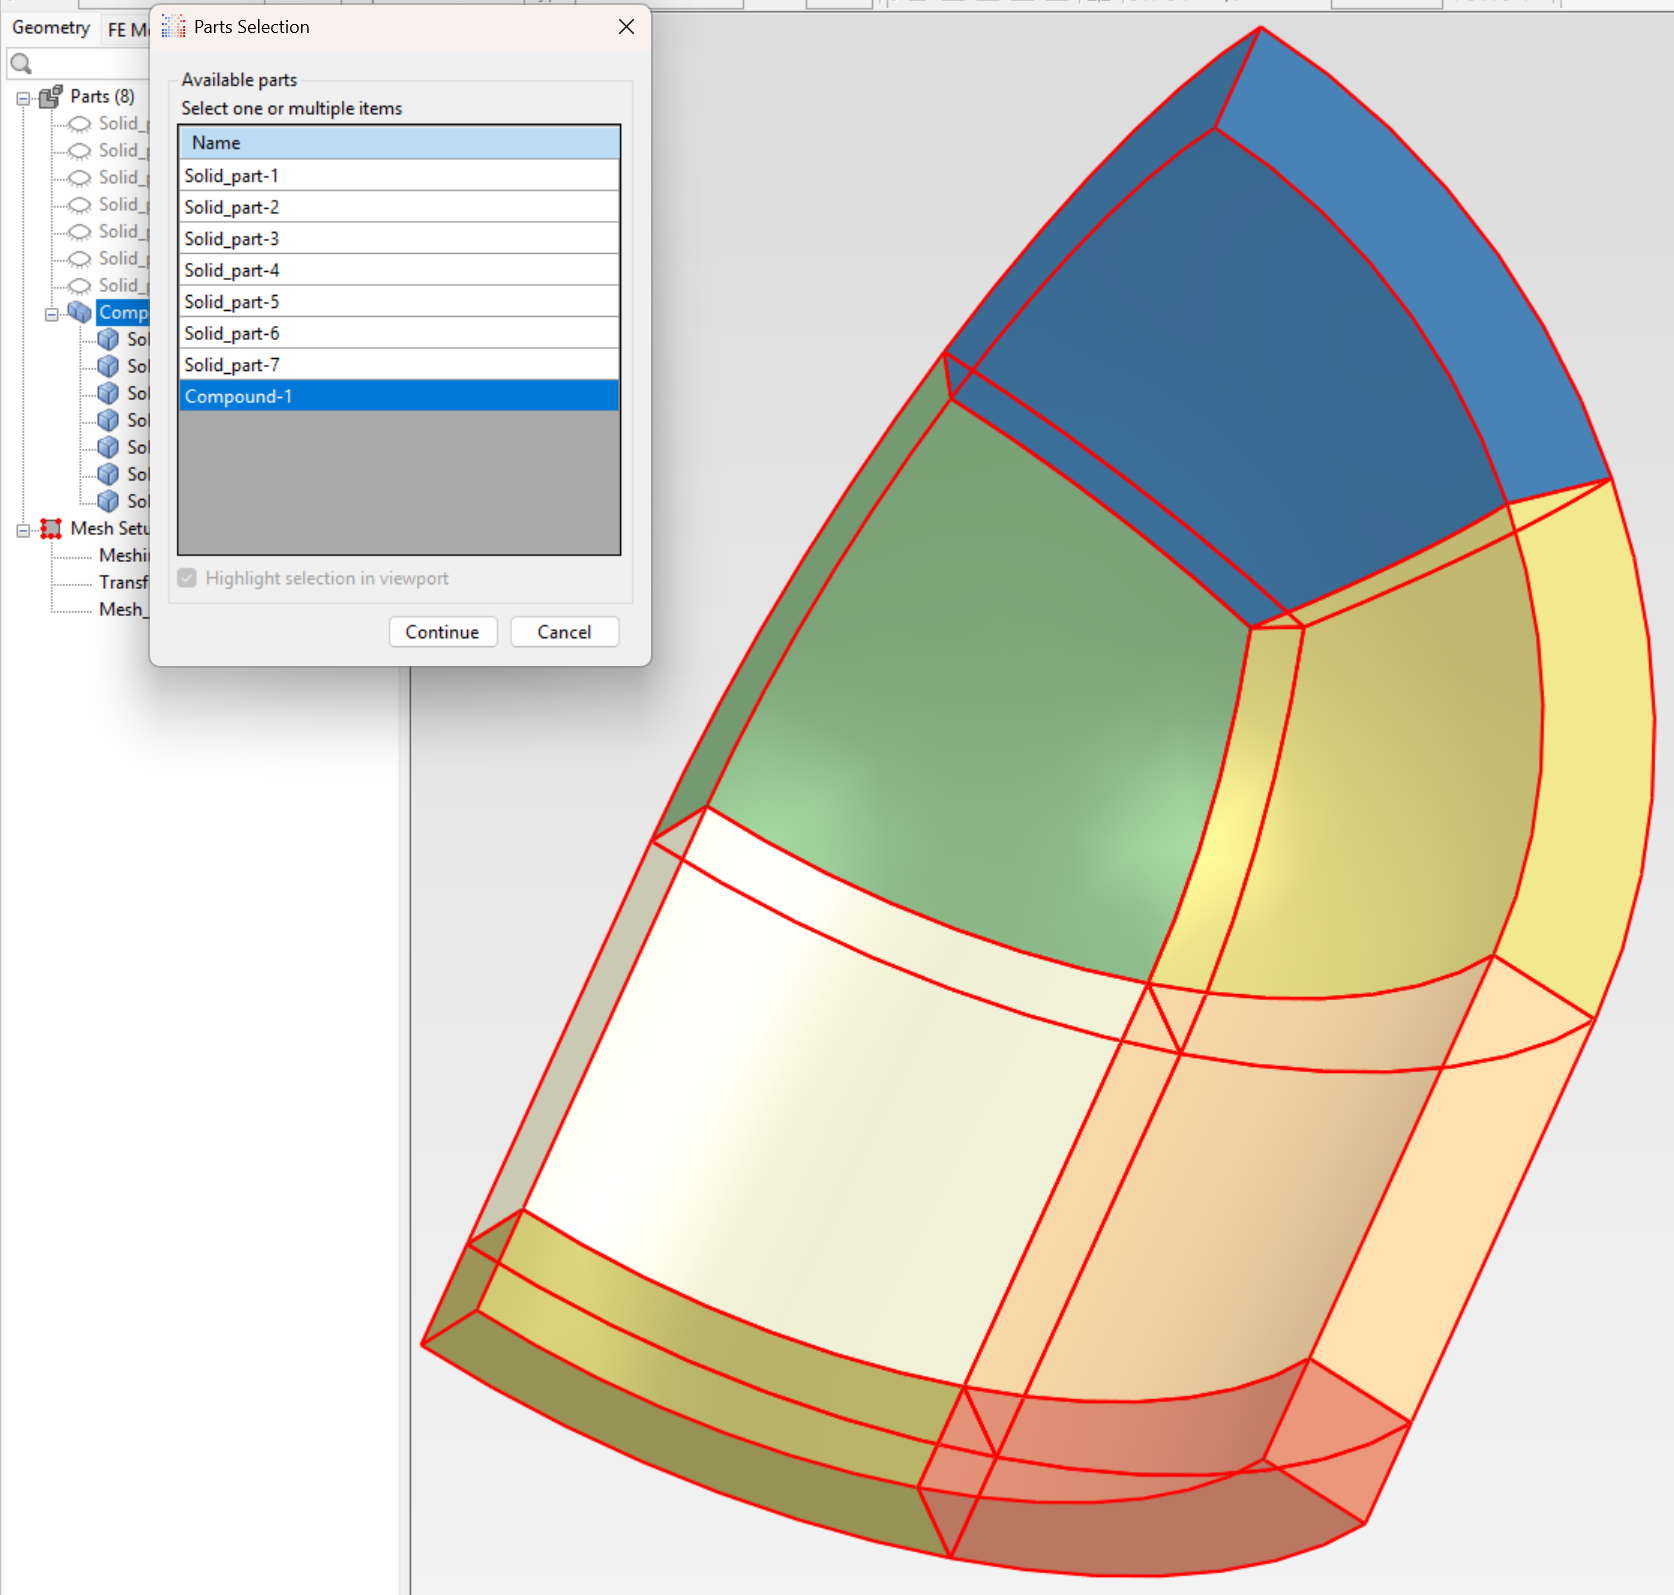
\includegraphics[keepaspectratio,scale=0.30]{images/sc10.png}}
            \only<2>{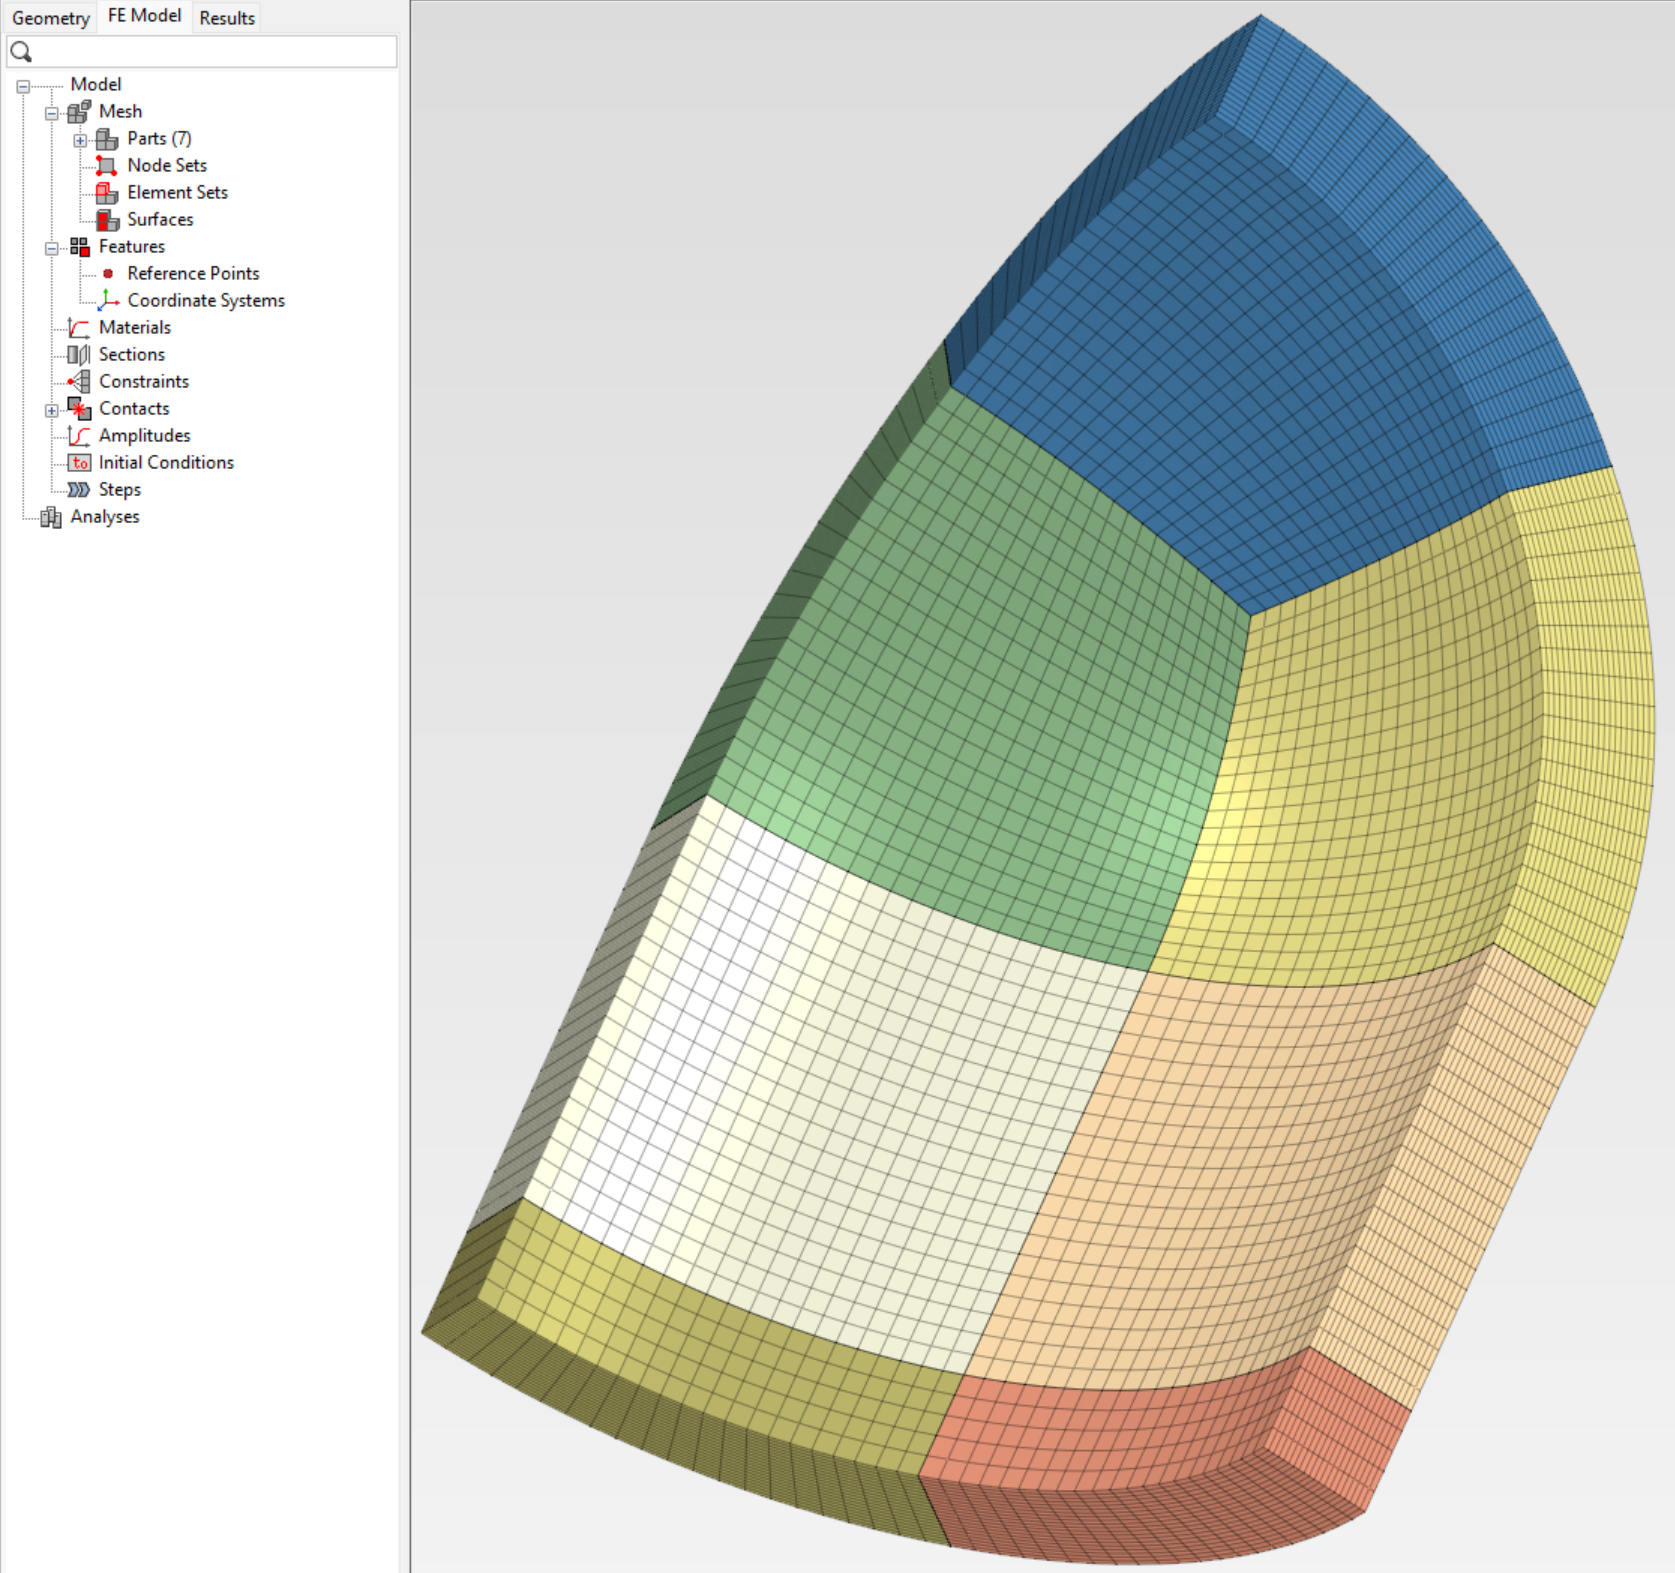
\includegraphics[keepaspectratio,scale=0.30]{images/sc11.png}}
            \caption{メッシュ設定の概要}
          \end{overlayarea}
        \end{center}
      \end{figure}
    \end{column}
  \end{columns}
  \only<1>{
    \begin{textblock*}{160pt}(200pt,73pt)
      \begin{tikzpicture}
         \node[rectangle,fill=cud_yellow,text width=90pt,text centered,rounded corners,minimum height=40pt](s) at (1cm,1cm) { \scriptsize メッシュ作成対象};
         \draw[->, draw=cud_red, line width=1pt] (10pt,50pt) -- (80pt,100pt);
      \end{tikzpicture}
    \end{textblock*}
  }
  \only<2>{
    \begin{textblock*}{160pt}(200pt,90pt)
      \begin{tikzpicture}
         \node[rectangle,fill=cud_yellow,text width=90pt,text centered,rounded corners,minimum height=40pt](s) at (1cm,1cm) { \scriptsize  1ヵ所の板厚方向の\\メッシュサイズ設定が\\全体に伝搬};
         \draw[->, draw=cud_red, line width=1pt] (50pt,50pt) -- (120pt,76pt);
      \end{tikzpicture}
    \end{textblock*}
  }
\end{frame}
